% !TeX encoding   = UTF-8
\documentclass[12pt]{article}

\usepackage{sbc-template}

\usepackage{graphicx,url}
\usepackage[brazil]{babel}
\usepackage[utf8]{inputenc}
\usepackage{graphicx}   %Package para figuras
\usepackage{enumerate}
\usepackage{tabularx}
\usepackage{multirow}
\usepackage[table,xcdraw]{xcolor}


\sloppy

\title{Ferramentas para Business Report \\
com Suporte à Linguagem XBRL - \\
Revisão Sistemática da Literatura}

%\author{Vagner Clementino\inst{1}}

\address{Departamento de Ciência da Computação\\
        Universidade Federal de Minas Gerais (UFMG)\\
%  \email{vagnercs@dcc.ufmg.br}
}

\date{Dezembro de 2015}
\begin{document}

\maketitle

%\begin{abstract}
%  This meta-paper describes the style to be used in articles and short papers
%  for SBC conferences. For papers in English, you should add just an abstract
%  while for the papers in Portuguese, we also ask for an abstract in
%  Portuguese (``resumo''). In both cases, abstracts should not have more than
%  10 lines and must be in the first page of the paper.
%\end{abstract}

\begin{resumo}
\end{resumo}


\section{Introdução}
\label{sec:contexto}

Uma \textit{Revisão Sistemática da Literatura} - SLR (do inglês Systematic Literature Review) é uma
metodologia científica cujo objetivo é identificar, avaliar e interpretar
\textit{toda} pesquisa \textit{relevante} sobre uma questão de
pesquisa, área ou fenômeno de
interesse\cite{keele2007guidelines,wohlin2012experimentation}. Por se tratar de uma metodologia científica deve estar amparada por um processo conciso para a sua correta execução. Neste sentido, trabalhos que descrevem boas práticas na condução de uma SLR salientam a necessidade da definição de um protocolo durante a fase de planejamento de uma Revisão \cite{keele2007guidelines, biolchini2005systematic}.

Neste contexto, o presente documento tem por objetivo propor um conjunto de diretrizes a serem seguidas durante a condução de uma Revisão Sistemática da literatura sobre o tema \textit{ferramentas para Relatórios de Negócio com suporte à linguagem XBRL}. \textit{Relatórios  de Negócio (Business Report)} é o produto final do  processo de divulgação pública de dados operacionais e financeiras de uma organização ou ainda a prestação regular de informações para os gestores dentro de uma empresa visado apoiá-los no processo de tomada de decisão.
\cite{lymer1999business}. Há uma terceira via da área de  Relatórios de Negócio está relacionada ao processo de prestação de contas por entes públicos aos governos nacionais. A XBRL (\textit{eXtensible Relatórios de Negócio Language}) é uma linguagem para divulgação e intercâmbio de informações financeiras baseada em XML\cite{xbrl_conceitos_aplicacoes}. O padrão vem sendo adotado por diversas instituições e empresas em todo mundo com o suporte de um consórcio global\footnote{\url{www.xbrl.org}} com mais de 650 membros que incentivam a criação de jurisdições locais. Atualmente o consórcio conta com 24 jurisdições, sendo que em países como  Estados Unidos, Grã-Bretanha e Austrália, a XBRL já é a linguagem oficial para entrega
de relatórios à órgãos de governo. A Figura \ref{fig:world_map} exibe os países que estão promovendo a adoção da XBRL. Estes países estão com a coloração mais escura no mapa.

\begin{figure}[htb]
\centering
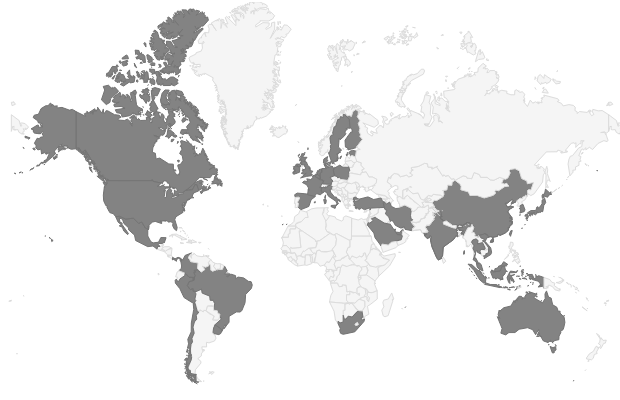
\includegraphics[width=.75\textwidth]{../img/world-map.png}
\caption{O uso da XBRL no mundo}
\label{fig:world_map}
\end{figure}

\section{Justificativa}
\label{sec:problema}

Tendo em vista determinação da Secretaria do Tesouro Nacional, órgão
vinculado ao  Ministério da Fazenda do Brasil, que definiu o XBRL como
padrão para o envio de relatórios de prestação de contas pelos entes
federativos (estados e municípios) por meio do SICONFI – Sistema de Informações Contábeis e Fiscais do Setor Público Brasileiro \cite{nt_03_2013}, surge a necessidade por parte
daquelas organizações do \textit{desenvolvimento ou aquisição} de sistemas de
informação capazes de criar, processar e enviar informações no formato
XBRL. Um cenário onde tal situação ocorre tal necessidade é latente é em
prefeituras de cidades de pequeno e médio porte que necessitam prestar contas
via \textit{XBRL}, contudo, não possuem conhecimento ou tempo necessário para desenvolver alguma ferramenta que suporte a linguagem.

Neste sentido, verifica-se que existe a demanda por parte das organizações, especialmente as entidades públicas, de referências de qualidade sobre o assunto de \textit{XBRL}. Neste contexto, entende-se que uma Revisão Sistemática da Literatura - SLR  que avaliasse as ferramentas para Business Report que dão suporte ao XBRL pode \textit{subsidiar a tomada de decisão} por parte dos gestores públicos sobre a aquisição de tais ferramentas. Além disso, um trabalho neste sentido poderia subsidiar o desenvolvimento de novas ferramentas que venham preencher as eventuais lacunas existentes nos sistemas atuais. Ademais, traz o foco da comunidade científica sobre um assunto que vêm crescendo bastante nos últimos anos, dentre outros motivos, devido à necessidade das organizações públicas ou privadas de serem cada vez mais transparentes.


\section{Metodologia de Pesquisa}
\label{sec:metodologia}

\subsection{Protocolo da Revisão}
\label{subsec:protocolo}

Uma \textit{Revisão Sistemática da Literatura} - SLR (do inglês Systematic Literature Review) é uma
metodologia científica cujo objetivo é identificar, avaliar e interpretar
\textit{toda} pesquisa \textit{relevante} sobre uma questão de pesquisa, área
ou fenômeno de interesse \cite{keele2007guidelines,wohlin2012experimentation}. Neste trabalho
será utilizada as diretrizes proposta \cite{keele2007guidelines} no qual uma
Revisão Sistemática deve seguir os seguintes passos:

\begin{enumerate}
  \item \textbf{Planejamento}
  \begin{enumerate}
    \item \textit{Identificar a necessidade da Revisão}
    \item \textit{Especificar questões de pesquisa}
    \item \textit{Desenvolver o Protocolo da Revisão}
  \end{enumerate}
  \item \textbf{Condução/Execução}
  \begin{enumerate}
    \item \textit{Seleção dos Estudos Primários}
    \item \textit{Análise da qualidade dos Estudos Primários}
     \item \textit{Extração dos Dados}
     \item \textit{Sintetização dos Dados}
   \end{enumerate}
  \item \textbf{Escrita/Publicação}
  \begin{enumerate}
    \item \textit{Redigir documento com os resultados da Revisão}
    \item \textit{Redigir documento com lições aprendidas}
  \end{enumerate}
\end{enumerate}

Conforme exposto, durante o planejamento da revisão deve desenvolvido um
protocolo com as diretrizes que conduzirão a pesquisa. Além disso devem ser
propostas as questões de pesquisa que devem ser respondidas pelo SLR. Para
esta revisão são propostas as seguintes questões de pesquisa:

\begin{itemize}

  \item \textbf{$Q1$}: Quais são as ferramentas para Relatórios de Negócio que
    suportam a XBRL?
  \item \textbf{$Q2$}: Quais são os atributos comuns as ferramentas
    que possibilitem a comparação entre elas?
  \item \textbf{$Q3$}: Existem casos reais de utilização da ferramenta
    (Estudos de Casos, Whitepapers e etc)?
  \item \textbf{$Q4$}: Qual setor da economia (governos, medicina, setor financeiro) a ferramenta possui histórico de utilização?

\end{itemize}
A partir deste conjunto de questões é possível propor as sentenças de busca que
serão utilizadas na busca dos estudos primários e subsidiar o processo de
extração dos dados daqueles estudos.

\subsection{Critérios de Inclusão e Exclusão}
\label{subsec:inclusao-exclusao}

Nesta seção define-se os critérios para a inclusão de determinado estudo
primário na Revisão. Naturalmente para o estudo ser incluído deverá atender as diretrizes propostas bem
como passar pelo crivo da avaliação de qualidade, conforme disposto na Subseção
\ref{subsec:analise-qualidade}. Neste sentido, um trabalho para ser aceito
como estudo primário deve atender aos seguintes critérios de inclusão:

\begin{itemize}

\item Tem ser publicado a partir de 2008.
\item Estar escrito em língua inglesa.
\item Artigos de Conferência, journals e Whitepapers
\item Dissertações ou Teses apenas se a ferramenta proposta tenha sido
  implementada e testada.
\end{itemize}


No de caso algum estudo recuperado atender qualquer um dos dos seguintes
critérios de exclusão ele deverá ser removido do Revisão mesmo que ele atenda a
algum outro critério de inclusão descritos acima. Os critérios de exclusão
deste trabalho são os seguintes:

\begin{itemize}
\item Trabalhos escritos em outra língua que não a inglesa
\item Documentos duplicados.
\item Livros
\item Dissertações ou Teses apenas se a ferramenta que não há a implementação da
  ferramenta.
\item Literaturas escritas antes do ano de 2008
\end{itemize}

\subsection{Seleção dos Estudos Primários}
\label{subsec:estudos-primarios}

Estudo Primário, no contexto da evidência, é um estudo empírico que investiga
uma questão de pesquisa específica\cite{keele2007guidelines}. No caso de um SLR são os estudos que
possibilitam responder as questões de pesquisa proposta na Revisão. Os guias de boas práticas na condução de uma Revisão Sistemática, especialmente
os da medicina, pregam a necessidade de uma busca exaustiva em diversos tipos
de bases de dados, sejam elas eletrônicas ou não. Não obstante, devido à
evolução das ferramentas de indexação de trabalhos acadêmicos, uma revisão pode
utilizar apenas base de dados eletrônicas sem perda de generalidade. Neste
trabalho, foram utilizadas as bases de dados constantes da Tabela
\ref{tab:base-dados}. Trata-se de uma lista com pequenas alteração da
proposta por \cite{Brereton2007571} com a inclusão de algumas bases,
especialmente o \textit{Google Scholar} e  \textit{XBRL Consortium}. No caso
\textit{Google Scholar} alguns trabalhos demostraram através de suas pesquisa é
possível encontrar 90\% dos artigos passíveis de serem descobertos em outras
bases de dados \cite{yasin2012quality}. Para a base de dados \textit{XBRL
  Consortium} a justificativa vem do fato que ser este o  site da entidade mantenedora do XBRL.

\begin{table}[ht]
\centering
\begin{tabular}{|c|l|c|c|}
\hline
\textbf{\#} & \multicolumn{1}{c|}{\textbf{Base de Dados}} & \textbf{Total} & \textbf{\%} \\ \hline
1           & IEEE Xplore                                 & 3              & 0,74\%      \\ \hline
2           & ScienceDirect                               & 100            & 24,57\%     \\ \hline
3           & Springer Link                               & 6              & 1,47\%      \\ \hline
4           & ACM Digital Library                         & 97             & 23,83\%     \\ \hline
5           & Web of Science                              & 9              & 2,21\%      \\ \hline
6           & CiteSeer                                    & 45             & 11,06\%     \\ \hline
7           & Wiley Online Library                        & 54             & 13,27\%     \\ \hline
8           & Scopus Elsevier                             & 8              & 1,97\%      \\ \hline
9           & EL Compendex                                & 9              & 2,21\%      \\ \hline
10          & Google scholar                              & 30             & 7,37\%      \\ \hline
11          & XBRL Consortium                             & 46             & 11,30\%     \\ \hline
\multicolumn{2}{|c|}{Total}                               & 407            & 100,00\%    \\ \hline
\end{tabular}
\caption{Base de dados e número de artigos}
\label{tab:base-dados}
\end{table}

Para obter o total de trabalhos exibidos na tabela \ref{tab:base-dados} cada
uma das bases de dados foi consultada com a sentença de busca ``XBRL \textbf{AND} Business Report \textbf{AND} tool
''. Com o objetivo de reduzir o número de documentos recuperados e melhorar a
qualidade dos resultados o seguintes critérios foram aplicados nas ferramentas
de busca: trabalhos publicados a partir de 2008 em que os termos pesquisados
estivessem no título, resumo ou nas palavras-chaves.

Após a primeira consulta realizada conforme descrito anteriormente, uma nova
rodada de consultas era realizada utilizando um \textit{Dicionários de Sinônimos}, que consiste basicamente de um conjunto de
termos similares aos originais que podem aumentar o leque de artigos
recuperados durante a busca. A Tabela \ref{tab:dicionario} exibe o dicionário
de dados que deverá ser utilizado durante a Revisão. A total deste processo foi
obtido um total de \textit{400} trabalhos recuperados.

\begin{table}[ht]
\centering
\resizebox{\textwidth}{!}{%
\begin{tabular}{|c|l|}
\hline
\multicolumn{2}{|c|}{\textbf{DICIONÁRIO DE SINÔNIMOS}} \\ \hline
\textbf{Termo Original} & \multicolumn{1}{c|}{\textbf{Sinônimo}} \\ \hline
XBRL & XML OR XHTML \\ \hline
tool & sofwtare OR  application OR product OR project OR development \\ \hline
Business Report & Finantial Report OR Data Extraction \\ \hline
\end{tabular}
}
\caption{Dicionário de Sinônimos}
\label{tab:dicionario}
\end{table}

\subsection{Decisão de Inclusão e Exclusão}
\label{subsec:decisao-inclusao}

Tendo em vista que os estudo primários foram selecionados de diversas bases de
dados (vide Tabela \ref{tab:base-dados}) ocorreram duplicação de
resultados. Para ajudar na tarefa de remoção de trabalhos duplicados foi utilizado a
ferramenta para a gestão de referências
\textit{JabRef}\footnote{\url{http://jabref.sourceforge.net/}}. Para cada uma
das bases de dados consultadas (Tabela \ref{tab:base-dados}) foi criado um
bando de dados na ferramenta no qual aplicada a funcionalidade de remoção de
duplicada. Trata-se de um processo automatizada cujo os detalhes fogem do
escopo deste texto. Todavia, para os casos em que o \textit{JabRef} não
consegui determinar se dois documentos são duplicados, a ferramenta solicita a
supervisão do usuário. Posteriormente todos os onze bancos de dados criados no
passo anterior foram mesclados em um único para o qual foi solicitada a remoção
de duplicatas. Aproveitando que a ferramenta \textit{JabRef} indentifica o tipo
de publicação do trabalho foram removidos os estudo identificados como livros.
Desta forma, ao final este processo o número de \textit{382} trabalhos.

Embora o título de um estudo nem sempre são descritivos o suficiente para
indicar o assunto de estudo, foi adotado o processo de remover os estudos
primários avaliando inicialmente o seu título. Ao final deste processo de
filtro foram \textit{excluídos 202 artigos}. Na terceira etapa, o resumo
(abstract) dos estudos foram utilizados como critérios de escolha. Esta é
última etapa antes da avaliação de qualidade dos estudos (Subseção
\ref{subsec:analise-qualidade}). Apesar da literatura ponderar a necessidade
deste processo de escolha ser realizado aos pares, este procedimento não foi
adotado tendo em vista a impossibilidade de outro pesquisador ou especialista
com a possibilidade de realizar tal tarefa. Ao final deste quatros passos
restaram um total de para serem avaliados segundo os critérios de qualidade
dispostos na Subseção \ref{subsec:analise-qualidade}. A Figura \ref{fig:fases}
exibe o número de trabalhos existentes em cada fase de seleção da Revisão.


\begin{figure}[htb]
\centering
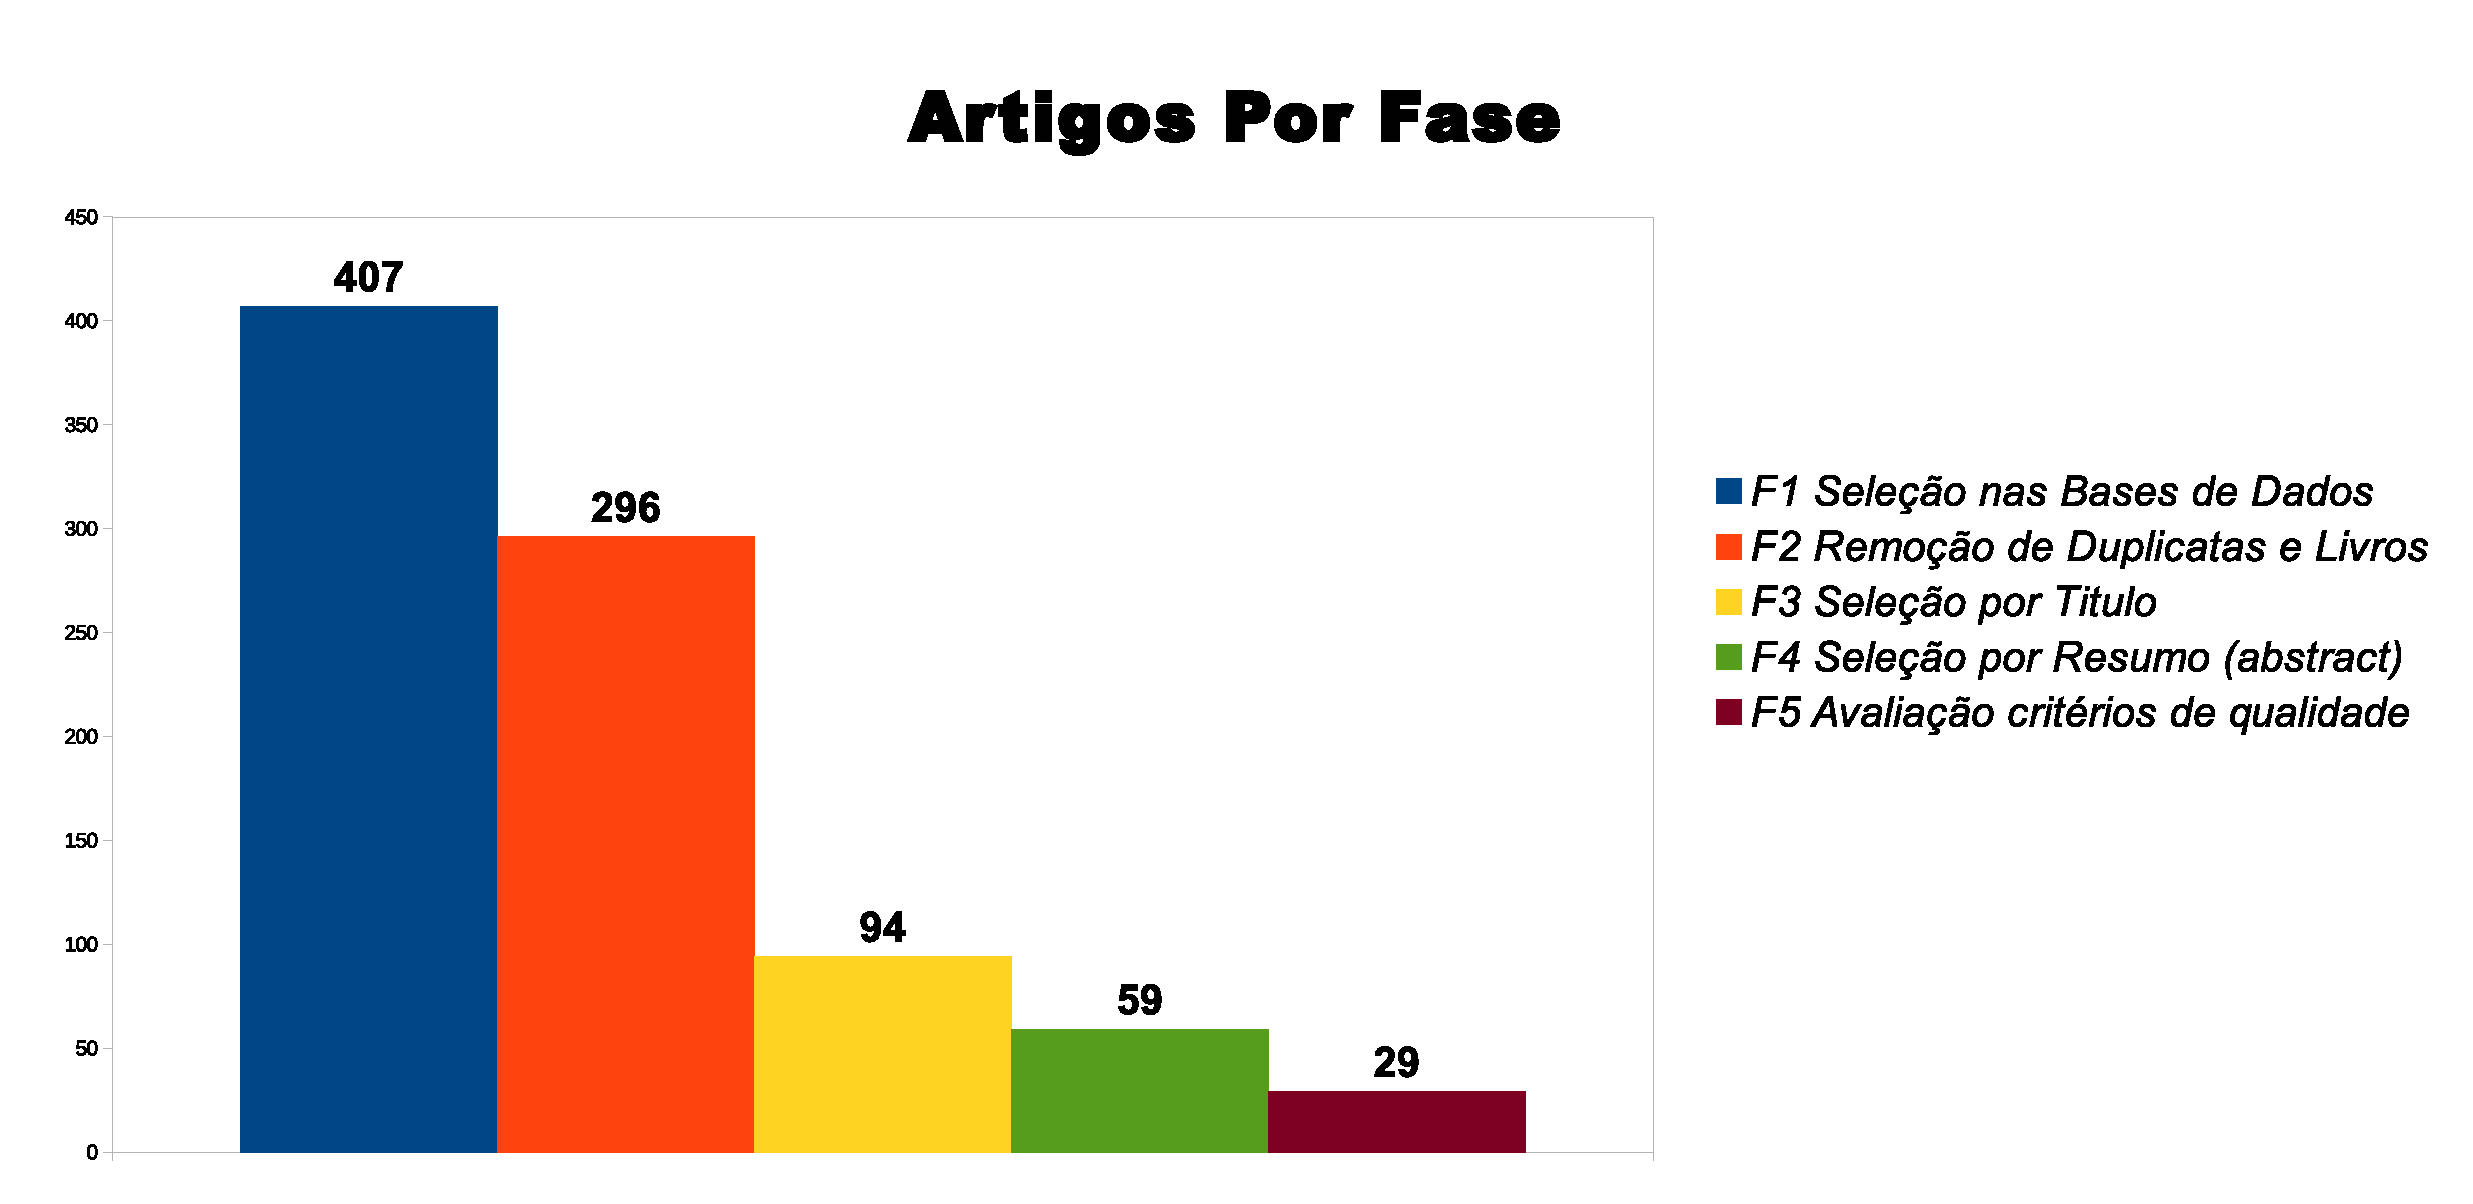
\includegraphics[width=.75\textwidth]{../img/graph_fases.eps}
\caption{Total de artigos em cada fase da SRL}
\label{fig:fases}
\end{figure}

\subsection{Análise de Qualidade}
\label{subsec:analise-qualidade}



\subsection{Extração dos Dados}
\label{subsec:extracao}

\subsection{Sintetização dos Dados}
\label{subsec:sintetizacao}

\section{Resultados}
\label{subsec:resultados}
\section{Limitações e Ameaças a Validade}
\label{sec:limitacoes}


\bibliographystyle{sbc}
\bibliography{../bib/slr_xbrl_tools}

\end{document}
